% For the listing caption reference
%! Suppress = UnresolvedReference

% To include word count of tables
%TC:group table 0 1

\chapter{Implementing Flexible Resource Allocation Environment and Server Agents}\label{ch:implementing-flexible-resource-allocation-environment-and-server-agents}
In order to implement the solution from chapter~\ref{ch:proposed-solution}, a Mobile Edge Cloud (MEC) computing network
must be simulated for both training and evaluation of agents. Due to the impractically of physically setting up
such a network and to train agents offline and in parallel. This chapter splits the implementation into three sections:
simulation of MEC networks (section~\ref{sec:simulating-mec-networks}), server auction and resource
allocation agents (section~\ref{sec:implementing-auction-and-resource-allocation-agents}) and the training of agents
(section~\ref{sec:training-agents}).

The implementation discussed below as written in Python and available to download from
Github~\footnote{\url{https://github.com/stringtheorys/Online-Flexible-Resource-Allocation}}.

\section{Simulating MEC networks}\label{sec:simulating-mec-networks}
While the aim of the environment is to accurately simulate MEC servers, the implementation of the environment must
allow agents to interact and train on the environment efficiently. Therefore it has been implemented
as an OpenAI gym~\citep{openaigym}, the de facto standard for implementing reinforcement learning environments by
researchers. However the standard specification must be modified due to the problem being multi-agent and multi-step.

An example of running the environment is in listing~\ref{lst:example_flexible_resource_env}. There are three
sections to the code: the first is the construction of an environment where the environment settings
are passed to determine the number of servers, tasks and their attributes. These attributes are determined using
uniform random numbers generator for values between maximum and minimum value for each variable. The second step is to
create the environment using the reset function returning a new environment state.
The state contains a task if one needs to be auctioned and a dictionary of servers to their current
allocated tasks. Using these states, each server can generate actions either using the auction agent or resource
allocation agent depending on if a task needs auctioning. The final part is to take a step using the server actions
that returns an updated server state, the rewards for the actions, if the environment is finished and extra information
from the steps taken. The reward is a dictionary of each of the servers with either the winning price for the auctioned
task or a list of tasks that have finished either because they ran out of time or completed early, depending on the
step taken.

\begin{lstlisting}[language=Python, frame=single, caption={Example code for running the environment}, captionpos=b,
                   label={lst:example_flexible_resource_env}]
# Load the environment with a setting
env = OnlineFlexibleResourceAllocationEnv('settings.env')

# Generate the environment state
server_state = env.reset()

for _ in range(1000):
    # Generate actions
    if server_state.auction_task:
        actions = {
            server: auction_agent.bid(state)
            for server, state in server_state
        }
    else:
        actions = {
            server: resource_allocation_agent.weights(state)
            for server, state in server_state
        }

    # Take environment step
    server_state, reward, done, info = env.step(actions)

    # If the environment is finished then reset it
    if done:
        server_state = env.reset()
\end{lstlisting}

\subsection{Weighted server resource allocation}\label{subsec:weighted-server-resource-allocation}
A particular complication of the environment is to distribute server resources due to the fact that the resource
allocation agents provide a resource weighting rather than the actual task resource usage. Because of this, a novel
algorithm was implemented to convert the weighting to the actual resources of each task.

To allocate the computational resources is relatively simple compared to allocating resources for both storage and
bandwidth. For computational resources, the algorithm checks first if the weighted resources is greater than the
quantity required for the task to finish the compute stage of the task. If this is true then the resources needed for the
task to complete the compute stage are allocated. However, this also means that the weighted resources available for each
task is increased due to a task not using all of its resources. Because of this, the checks are repeated until no task
can be finished with its weighted resource within this time step. For the remaining task, they are just allocated their
weighted compute resources.

For allocating storage and bandwidth, this is more difficult due to the fact that when the server is still
loading the task, the server is allocating both storage and bandwidth resources while also allocating bandwidth
resources to tasks to send results back to users. Because of this, a tension exists between allocating bandwidth and
storage resources for all of the tasks fairly. The algorithm was therefore chosen to gives priority when allocating
resources to the tasks sending results as these tasks that are more likely to finish and to not penalise the
server by failing to complete the task within its deadline.

To allocate resources, a similar function to used to the one for allocating compute resources. First a check if done
using the weighted bandwidth resources to see is any task sending results will be finished with the resources.
This process is also repeated for the tasks loaded onto a server with the additional check that there is enough
available storage for the new data to be added. For any remaining task, this process is repeated until all of the
available resources are allocated in the time step. As a results, using this algorithm, the converting between
weightings to the actual resources usage allows for near maximum allocation of a server's available resources.

\section{Server auction and resource allocation agents}\label{sec:implementing-auction-and-resource-allocation-agents}
%% FIXME
%% Outline the task pricing and resource allocation agents

A range of different reinforcement learning techniques have been implemented, outlined in
Table~\ref{tab:reinforcement_learning_algorithms}, in order to explore the different options that a server would have
available to learn its policies. These policies were originally attempted to be implemented using
Tf-Agent~\citep{tf-agent} and a range of other frameworks with algorithm pre-programmed however due to numerous issues
that was not possible to do. Therefore all of the algorithm have been handcrafted using
tensorflow~\citep{tensorflow2015-whitepaper}, a Python module developed by Google, that gives the ability to construct
neural networks, backpropagation with custom loss functions and more.

Both deep Q networks and policy gradient algorithms are based on the Q function (explained in
section~\ref{sec:reinforcement-learning})) which tries to approximate the reward at the next time step. To do
this requires a reward function and a next observation to compare to in order to train these agents. The agent's
reward function and agent training observations are detailed in subsection~\ref{subsec:agent-rewards-functions}
and~\ref{subsec:agent-training-observations}.

A particular problem that this project encounter was with using recurrent neural network. This was because the
number of inputs were not fixed which means that during training, a minibatch was not possible as most of the inputs
all had different input lengths and tensorflow required all inputs to have a known, fixed length. Originally this was
sidestepped by calculating the loss for each input individually then finding the mean loss and gradient to update the
networks. However this was found to be computationally impractical requiring over two days to train an single agent
over 500 episodes. Because of this, a solution was found by padding all the inputs to be the same size using the
tensorflow preprocessing module with the sequence.pad\_sequence function. As a result, training became significantly
faster making large scale testing practical within a more reasonable time period of 16 hours for 600 episodes.

\subsection{Agent Rewards Functions}\label{subsec:agent-rewards-functions}
As explained in the background review for reinforcement learning (section~\ref{sec:reinforcement-learning}),
the Q values is the estimated discounted reward in the future for an action given a particular state. Therefore the
rewards that an agent receives for taking an action is extremely important to enable the agent to learn a predictable
reward function. This problem of complex reward functions are a known problem for DQN agent to deal with~\citep{atari}
that policy gradients agents can deal with this better due its ability directly learning the action
policy~\citep{Sutton1998}.

For the auction, the reward is based on the winning price of the task which is award for the winning. If the
task fails, the reward is instead multiplied by a negative constant in order to discourage the auction agent from
bidding on tasks that wouldn't be able to complete. As the price of zero is treated as a non-bid in the auction, the
agent gets a reward of zero in order to not penalise the agent. However, if the agent does bid on a task however
doesn't win, the agent's reward is set just below zero at -0.05 as a way of encouraging the agent to change their bid
but not large enough to force it to do so. \\
This reward is awarded at the time step of the auction instead of when the task fails or is completed as this makes the
function harder to learn as the auction agent has no control or observations over the resource allocation for a task at
that point.

For resource allocation, the reward function is much simpler than the auction agent's reward function, as it only needs
to consider the task being weighted at the time and rewards from other tasks allocated at the same time step. This is
because a task must consider its actions in conjunction with the resource requirements of other allocated tasks. \\
For successfully finishing a task, the reward is 1 while the reward if the task has failed is -1.5. This makes
failing a task more costly than completing a task. But when a task's action is not under consideration, this reward is
multiplied by 0.4 as while this rewards impact the task, their value is not as impactful as the reward for the action
on a particular task. These rewards don't consider the price payed for the task instead valuing each task equally with
the aim of finish all tasks not just the valuable ones. Using this information,
the reward function is simply the sum of the rewards of the finished tasks in the next time step.

\subsection{Agent Training Observations}\label{subsec:agent-training-observations}
In order to update both DQN and DDPG critic networks, the Q learning equation is used (equation~\eqref{eq:q_learning})
requires the next observation to evaluate the next Q value. However the next observation for an
agent is not clear as shown in figure~\ref{fig:environment-observations}. For both the auction and resource allocation
agents, there is an unknown number of actions taken by the other agents before its next observation is known.

\begin{figure}[h]
    \centering
    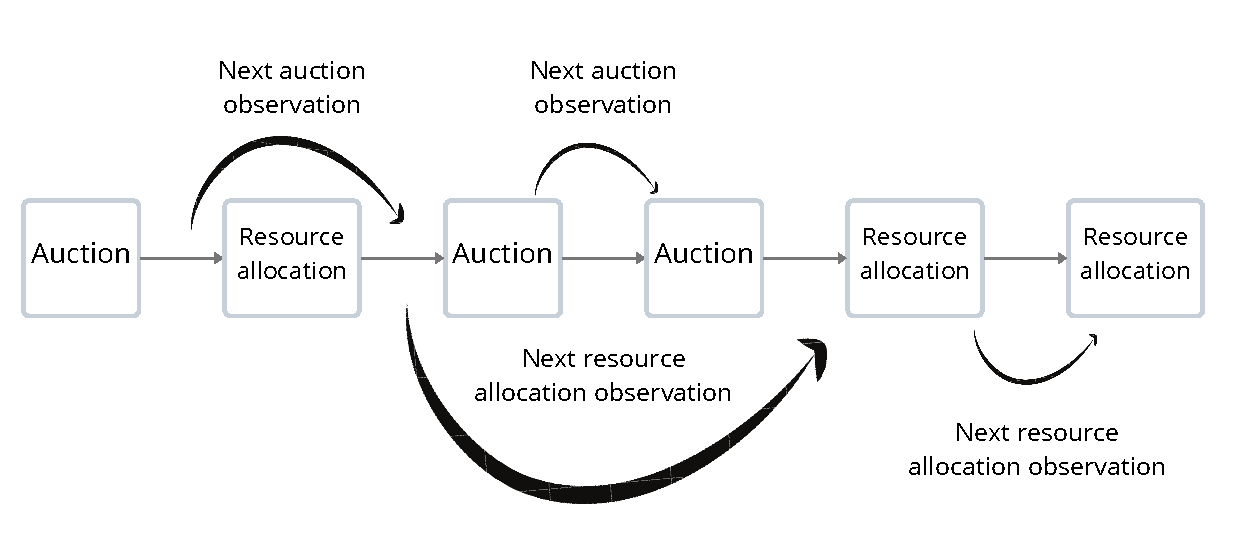
\includegraphics[width=14cm]{figures/4_implementation_figs/env_server_agents_observations.pdf}
    \caption{Environment server agents observations}
    \label{fig:environment-observations}
\end{figure}

For the resource allocation agent, a trick is implemented such that the next observation for the agent is not the
actual next resource allocation observation as shown in figure~\ref{fig:environment-observations} but a generated
observation from the resulting server state due to agent's actions. This is identical to the last case in the figure
where no auction occurs between resource allocation steps. Because of this, the resource allocation Q value is able to
approximate the reward for the results state of its actions directly making it appear to the agent during training that
there is no auction steps between observations.
% Todo add number of tasks observations problems

For the auction agent, as the agent observations require an auction task to select an action (the task bidding price).
A trick like the one implemented for the resource allocation agent can't be implemented. Therefore during training,
each server's last observation is recorded, such that when the next auction occurs, this new task observation can be
used as the server's next observation. This is a suboptimal solution for the agent as the next observation
has an unknown number of resource allocation steps resulting in changes to the current allocated tasks.
A possible solution that has not been implement in this project is n step prediction~\citep{multi-step-dqn}. Where the
agent doesn't predict the Q value of the next environment, but the value in n steps time. This approach could help
reduce the amount of randomness in the server's observations and improve bidding performance.

\section{Training agents}\label{sec:training-agents}
The first section of this chapter allowed for simulating MEC servers
(section~\ref{sec:simulating-mec-networks}) as a reinforcement learning environment. While the second
section implements auction and resource allocation agents that can interact with the proposed environment in order
to allow for the training of agents using a range of algorithms outlined in
Table~\ref{tab:reinforcement_learning_algorithms}.

Neural networks, the basis of the reinforcement learning agents implemented, often require huge amounts of data and
high powered GPUs to run efficiently. Because of this, Iridis 5, University of Southampton's supercomputer was utilised
with GTX1050 GPUs to train these agents for long periods of time and en mass. During training, for each episode a
random environment was generated from a list of possible settings so that the agents would be allocated to random
servers. The environment was run until a fixed set time step, with the agent observation being added to their replay
buffers after each actions that were chosen epsilon greedily.

After every 5 episodes, the agents would be evaluated using a set of environment that were pre-generated and
saved at the beginning of training. This allowed the same environments to be used over training in order to have a
consistent basis in order to compare the agents over time.

A table of agent hyperparameters can be found in \hyperref[app:agent-hyperparameter]{Appendix C}.

